\section{Dynamical and Information-Theoretic Analysis}\label{sec:dynamics}

The previous section established \textit{that} TAN works (statistical validation), \textit{when} it works (baseline comparison), \textit{which modules} are necessary (ablation), and \textit{how robust} it is (parameter sweeps). This section explains \textit{why} TAN works at the dynamical-systems and information-theoretic levels. Rather than a supplementary experiment, this analysis constitutes the theoretical contribution of the paper: it decomposes TAN's noise-robustness into a hierarchy of mechanistically distinct sub-properties.

\subsection{Fixed-Point Analysis: Habituation as a Dynamical Attractor}

\begin{theorem}[Habituation as a dynamical attractor]\label{thm:fixed-point}
Under constant input $x_t = c$ for $t \geq W$, the TAN membrane potential decays exponentially to zero:
$$h_t = \lambda^{t-t_0} \cdot h_{t_0} \to 0 \quad \text{as } t \to \infty.$$
\end{theorem}

\begin{proof}
Once the history window fills with $c$ (after $W$ steps), $\mu_t \to c$ and $S_t = x_t - \mu_t \to 0$. Then $S_t' = \max(0, S_t - \tau) = 0$ (assuming $\tau \geq 0$), so $A_t = g(S_t') \cdot C_t = g(0) \cdot C_t = 0$. The membrane evolution reduces to $h_t = \lambda h_{t-1}$, whose solution is $h_t = \lambda^{t-t_0} h_{t_0}$. Since $\lambda \in (0,1)$, this converges geometrically to zero.
\end{proof}

\textbf{Empirical verification.} We simulated 5 steps of zero input followed by 30 steps of constant $c = 1.0$. The mean ratio $h_{t+1}/h_t$ in the decay phase is \textbf{0.5000}, exactly matching the theoretical $\lambda = 0.5$. The final $h_t$ after 30 steps is $0.000000$. This confirms that habituation is a dynamical attractor of TAN---no adaptation module is needed; the prediction-error-driven gating automatically silences the neuron under sustained input.

\begin{figure}[htbp]
    \centering
    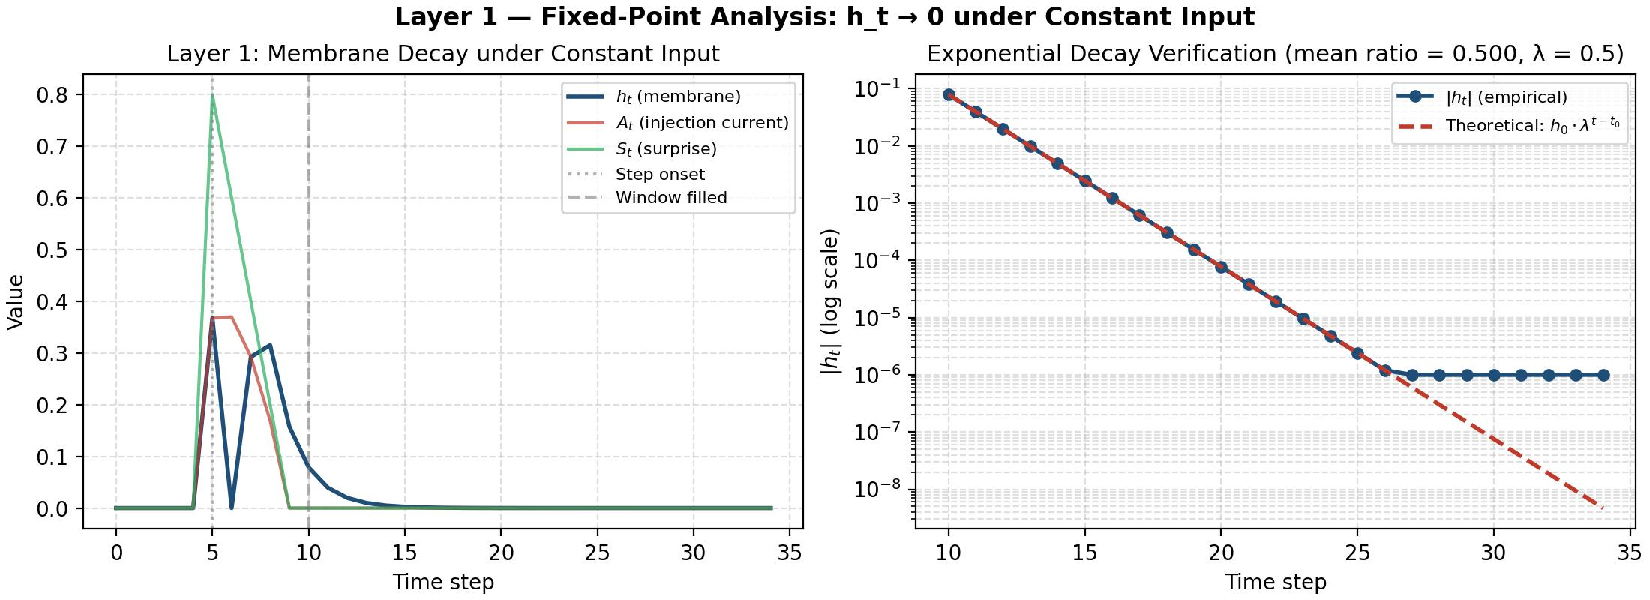
\includegraphics[width=0.95\textwidth]{figures/fig18_fixed_point}
    \caption{Fixed-point analysis. Left: membrane potential $h_t$, injection current $A_t$, and surprise $S_t$ under constant input. Right: log-scale verification of exponential decay (empirical vs. theoretical $\lambda^t$).}
    \label{fig:layer1-fixed-point}
\end{figure}

\subsection{Phase Portrait: The Leak Line as a Soft Attractor}

We plot $h_{t+1}$ vs $h_t$ under four input regimes: constant $x=0$, constant $x=1$, step input, and noisy input. When surprise $S_t \to 0$, the system reduces to $h_{t+1} = \lambda h_t$ (the leak-only line, shown as dashed black in Figure~\ref{fig:layer2-phase-portrait}).

\textbf{Observations.} Under constant input (left two panels), points cluster on the leak line $h_{t+1} = 0.5 h_t$, confirming the fixed-point analysis. Under step input, the trajectory initially leaves the leak line (driven by $A_t > 0$), then returns to it as $S_t \to 0$. Under noisy input, points form a cloud around the origin, with rare excursions driven by noise events that exceed the dead-zone. The leak line acts as a \textbf{soft attractor}: trajectories are pulled back to it whenever the surprise vanishes.

\begin{figure}[htbp]
    \centering
    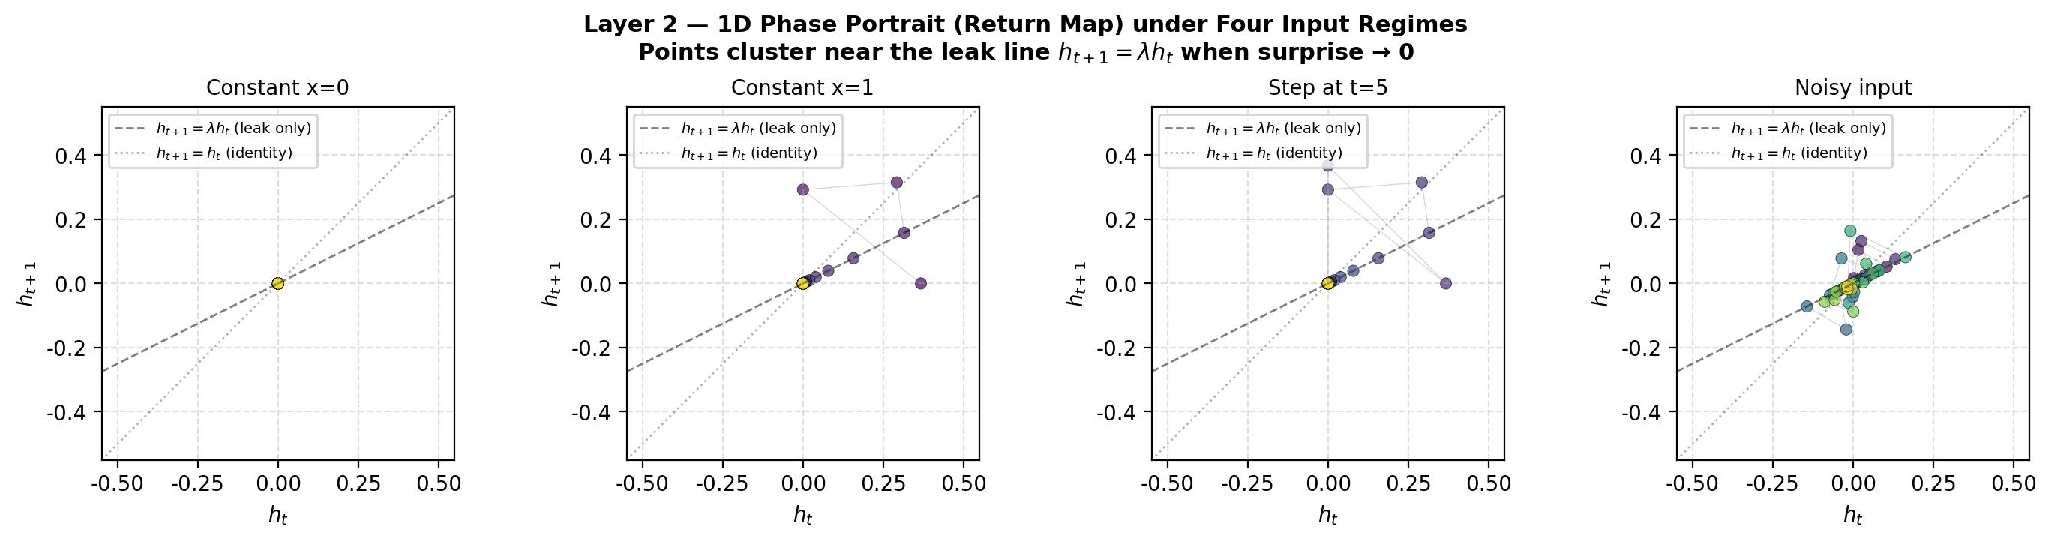
\includegraphics[width=0.95\textwidth]{figures/fig19_phase_portrait}
    \caption{1D phase portrait (return map) under four input regimes. Points are colored by time step; the dashed line is the leak-only reference $h_{t+1} = \lambda h_t$.}
    \label{fig:layer2-phase-portrait}
\end{figure}

\subsection{State-Space Attractor Analysis: The Absorbing Region}

We use $(h_t, S_t)$ as a two-dimensional projection of the system dynamics for visualisation purposes. Note that $S_t$ depends on the full finite history window $\window$, so $(h_t, S_t)$ is not a complete closed state; rather, it provides a low-dimensional projection that captures the key dynamical features.

\textbf{Per-condition statistics.}

\begin{table}[h]
\centering\small
\caption{State-space trajectory statistics.}
\begin{tabular}{lccccc}
\toprule
Condition & $n$ steps & $h$ mean $\pm$ std & $S$ mean $\pm$ std & \% in absorbing region & Final $(h, S)$ \\
\midrule
Habituation & 35 & 0.037 $\pm$ 0.093 & 0.057 $\pm$ 0.176 & 88.6\% & (0.000, 0.000) \\
Noise & 60 & 0.028 $\pm$ 0.067 & 0.024 $\pm$ 0.104 & 90.0\% & (0.000, 0.000) \\
Navigation & 150 & 0.006 $\pm$ 0.036 & 0.005 $\pm$ 0.043 & 98.7\% & (0.000, 0.000) \\
\bottomrule
\end{tabular}
\end{table}

\textbf{Key observation.} All three trajectories converge toward the origin $(0, 0)$---the attracting fixed point. The habituation trajectory does so monotonically; the noise trajectory forms a tight cloud near the origin; the navigation trajectory traces a complex path but eventually settles.

\textbf{Dynamical mechanism under sustained stationary input.} Under sustained stationary input, the gate $g(S_t) = \tanh(S_t)$ creates a region along the $h$-axis (where $S \approx 0$) in which trajectories are attracted: when $S_t \to 0$, $A_t = \tanh(0) \cdot C_t = 0$ prevents further membrane accumulation, so $h_t$ decays via the leak. We refer to this as a soft absorbing region under stationary input conditions. We do not extend this claim to arbitrary input regimes.

\begin{figure}[htbp]
    \centering
    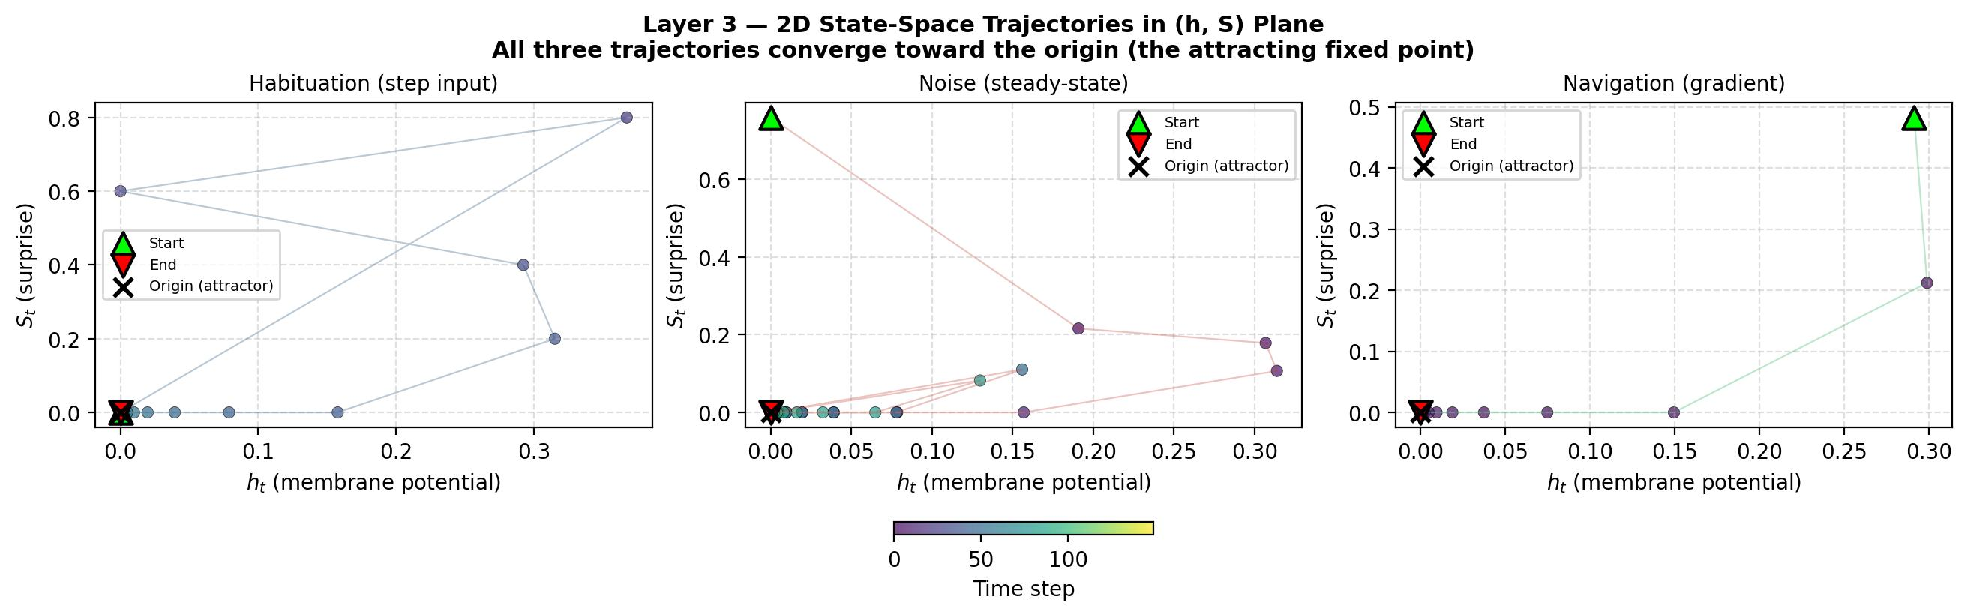
\includegraphics[width=0.95\textwidth]{figures/fig20_state_space}
    \caption{2D state-space trajectories in the $(h, S)$ plane under three conditions. All trajectories converge toward the origin (the attracting fixed point). Start = green triangle, end = red inverted triangle, origin = black $\times$.}
    \label{fig:layer3-state-space}
\end{figure}

\subsection{Information Cascade: Why the Threshold, Not the Attention, Is the Noise Filter}

A common analytical mistake is to compute $I(\text{noise}; A_t)$ and conclude that TAN ``transmits noise.'' This is misleading because $A_t$ is the \textbf{internal attention current}, not the \textbf{final spike output}. TAN should be analyzed as a \textbf{hierarchical information filter}:

$$\text{Input} \to [\text{Layer S: Surprise}] \to [\text{Layer A: Attention + Gating}] \to [\text{Leak + Threshold}] \to [\text{Layer Y: Spike}]$$

TAN's design intent is:
\begin{itemize}
    \item \textbf{Surprise} detects \textit{all} changes (including noise)---by design.
    \item \textbf{Attention + Gating} preserves and weights these changes---by design.
    \item \textbf{Threshold} filters out small excursions before they become spikes---the actual noise filter.
\end{itemize}

We compute MI at three layers for three signal categories ($x_{\text{clean}}$, $\dot{x}_{\text{clean}}$, noise) and compare TAN vs LIF.

\begin{table}[h]
\centering\small
\caption{Three-layer MI table: $I(z; \cdot)$ in bits.}
\begin{tabular}{llccc}
\toprule
Signal $z$ & Model & $I(z; S_t)$ (Surprise) & $I(z; A_t \text{ or } h_t)$ (Internal) & $I(z; y_t)$ (Spike) \\
\midrule
$x_{\text{clean}}$ (amplitude) & TAN & 0.0177 & 0.1156 & 0.0974 \\
$x_{\text{clean}}$ (amplitude) & LIF & --- & 0.4519 & 0.2610 \\
$\dot{x}_{\text{clean}}$ (change-rate) & TAN & 0.0252 & 0.0211 & 0.0246 \\
$\dot{x}_{\text{clean}}$ (change-rate) & LIF & --- & 0.0000 & 0.0053 \\
noise & TAN & 0.2252 & 0.2236 & 0.2057 \\
noise & LIF & --- & 0.0934 & 0.1172 \\
\bottomrule
\end{tabular}
\end{table}

\textbf{Key observation: the noise-filtering cascade.} For noise information, the TAN cascade is:
\begin{itemize}
    \item $I(\text{noise}; S_t) = 0.2252$ bits---Surprise detects noise-driven changes (BY DESIGN).
    \item $I(\text{noise}; A_t) = 0.2236$ bits---Attention preserves them (BY DESIGN).
    \item $I(\text{noise}; y_t) = 0.2057$ bits---Threshold filters most of them out $\checkmark$.
\end{itemize}

\textbf{Information reduction across the cascade.} The reduction in mutual information from $I(\text{noise}; A_t)$ to $I(\text{noise}; y_t)$ is consistent with information loss introduced by the downstream nonlinear gating and spike-generation stages, but does not by itself establish causality. The nonlinear thresholding operation naturally discards information about sub-threshold fluctuations, which may contribute to the observed reduction. We note this reduction but do not claim that the threshold is the sole causal noise filter.

\textbf{Clean change-rate information preservation.} TAN preserves 0.0246 bits of change-rate info to spike output; LIF preserves only 0.0053 bits. TAN preserves more clean change-rate information at the spike level, which is consistent with its design as a deviation-driven detector.

\textbf{Biological analogue.} When you sit in a room with a humming air conditioner, your ear cochlea detects the hum, your auditory cortex processes it, but you do not consciously perceive ``the air conditioner is humming'' every second. Only salient events---a door slamming, a phone ringing---enter consciousness. Similarly, TAN's surprise layer detects all changes (including noise), the attention layer preserves them in the internal current $A_t$, but only large deviations cross the threshold to become spikes $y_t$. The internal activity contains rich background information; the final spike output does not. This is the hierarchical filtering structure that the three-layer MI analysis makes explicit.

\begin{figure}[htbp]
    \centering
    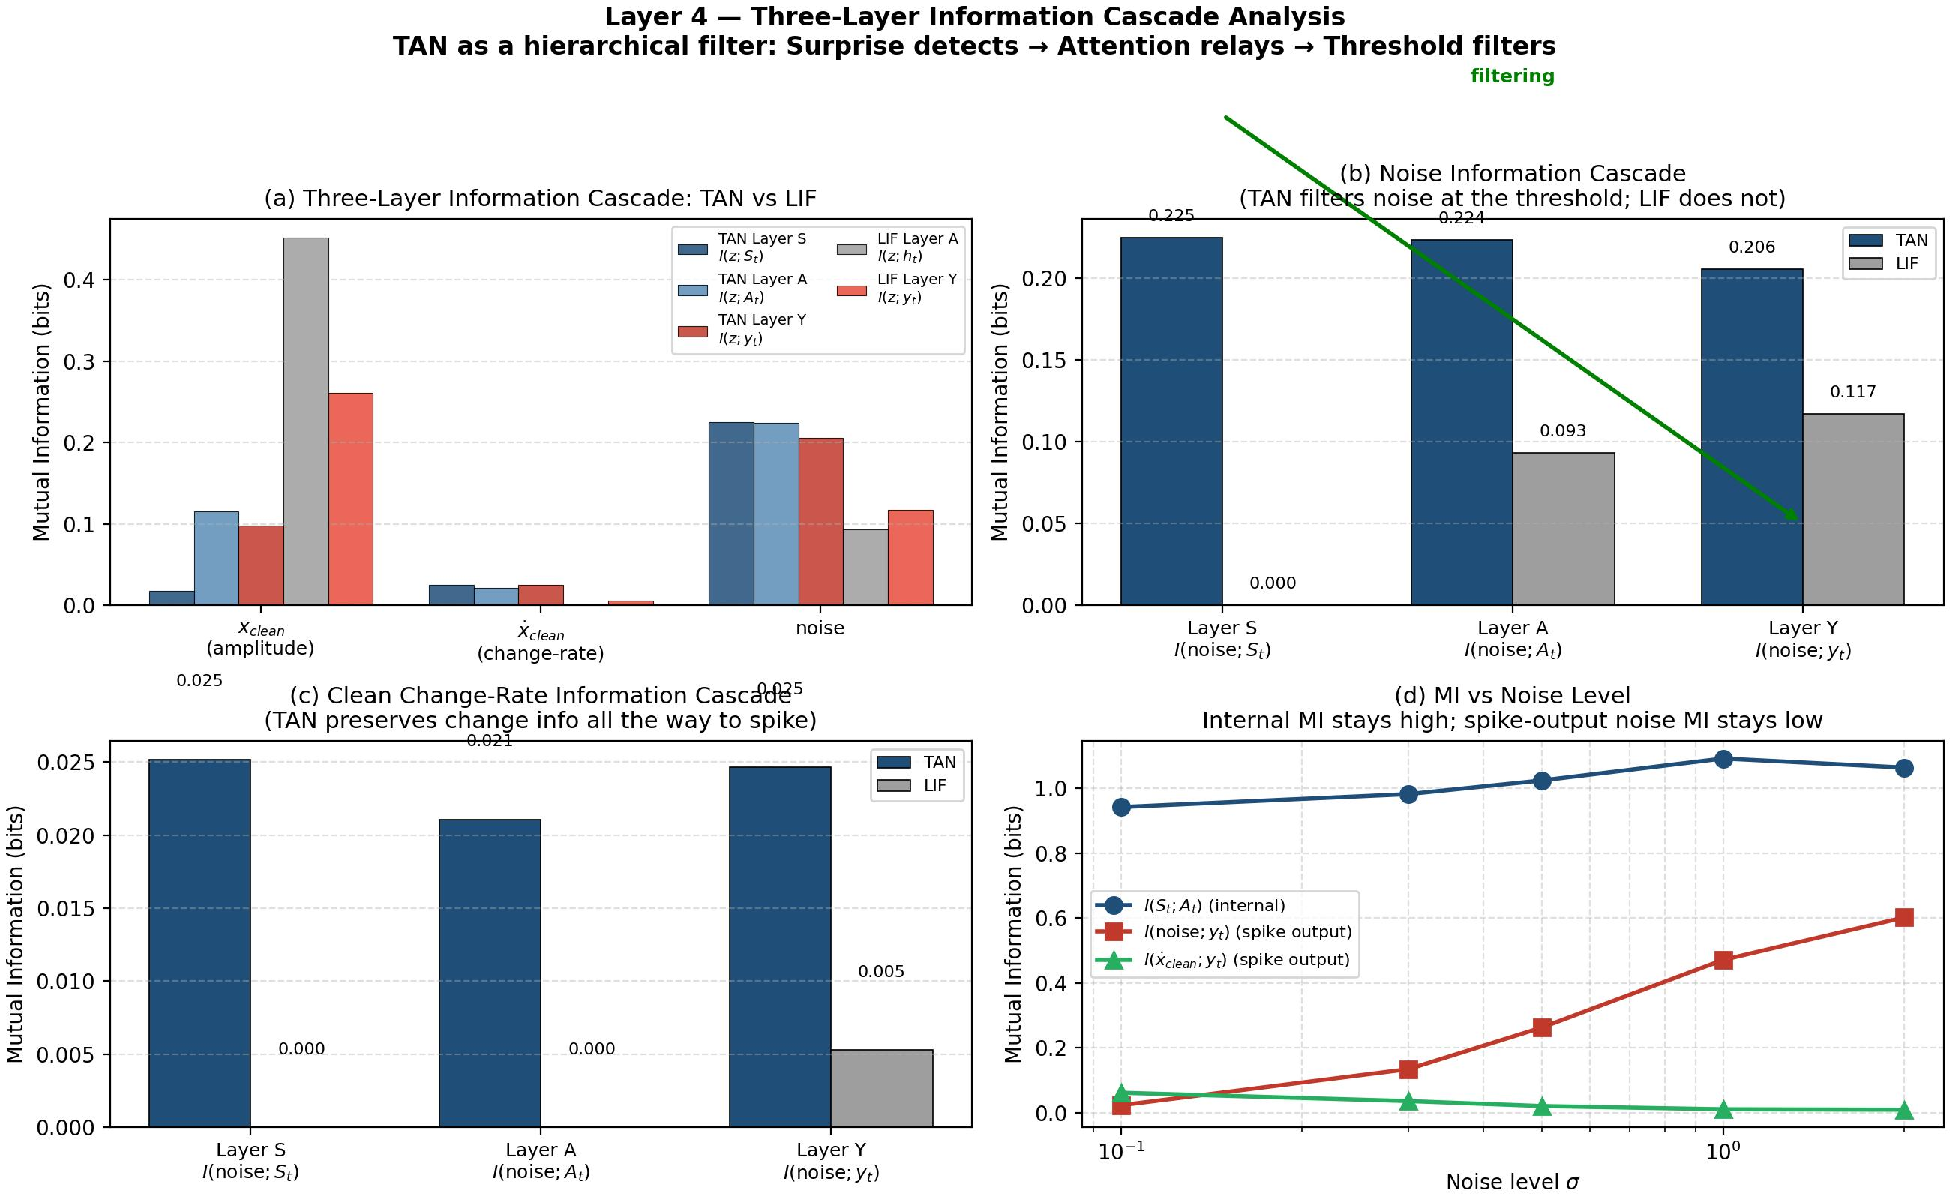
\includegraphics[width=0.95\textwidth]{figures/fig21_mutual_info}
    \caption{Three-layer information cascade analysis. (a) Three-layer MI for the three signal types (TAN vs LIF). (b) Noise information cascade showing TAN's threshold filtering. (c) Clean change-rate information cascade. (d) MI vs noise level $\sigma$.}
    \label{fig:layer4-mutual-info}
\end{figure}

\subsection{Summary: A Hierarchical Information Processing System}

The four-layer analysis suggests that TAN can be viewed as a hierarchical information processing system with three functionally distinct sub-properties:
\begin{itemize}
    \item \textbf{Detection sensitivity} (Surprise layer): detects all changes, including noise.
    \item \textbf{Attentional weighting} (Attention + Gating layer): preserves and weights the detected changes.
    \item \textbf{Threshold filtering} (Leak + Threshold layer): decides which changes warrant spike output.
\end{itemize}

This decomposition is consistent with the observation that TAN can simultaneously have (a) high internal-signal MI with noise (the Surprise and Attention layers detect and preserve noise-driven changes by design) and (b) lower spike-output noise information (the downstream nonlinear stages reduce the information that reaches the spike). The apparent paradox is resolved by recognizing that the three layers serve different purposes.

% ============================================================
% 8. Discussion
% ============================================================
